\documentclass[]{scrartcl}
\usepackage[]{algorithm2e}
\usepackage{xcolor}
\usepackage{graphicx}
\usepackage{listings}
\definecolor{comment}{rgb}{0,0.5,0}
%opening
\title{Ising Model}
\author{Danny Goldstein}

\begin{document}
	
	\maketitle
	
	\section{Introduction}
	
	The 2D Ising model is one of the simplest statistical models to show a phase transition \footnote{Gallavotti, G. (1999), Statistical mechanics, Texts and Monographs in Physics, Berlin: Springer-Verlag, doi:10.1007/978-3-662-03952-6, ISBN 978-3-540-64883-3, MR 1707309}. The purpose of this simulation is to investigate how some properties of this model change across the phase transition. The Ising model is a simple model for studying magnetism in materials. We are writing this simulation to study the how the magnetism, magnetic susceptibility, heat capacity and hysteresis change across the phase transition.
	
	
	\section{Mathematical Model}
	This model consists of a lattice of spins. Spins represent magnetic dipole moments, and the lattice of these spins represents a magnetic material. See Figure \ref{fig:cartoon1} for a cartoon.

\begin{figure}[ht]
	\centering
	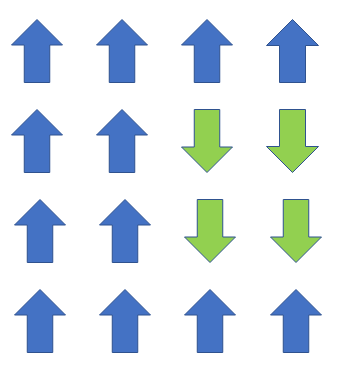
\includegraphics[width = 0.5\linewidth]{IsingCartoon}
	\caption{Cartoon of a 4x4 lattice of spins}
	\label{fig:cartoon1}
\end{figure}
	
	We define a spin on lattice site $i$ as $\sigma_i \in \{+1, -1\}$.
	The Hamiltonian for this system is then 
	$$H = -\sum_{\langle i \;  j \rangle} J_{i,j} \sigma_i \sigma_j -\sum_i \sigma_i h_i$$
	
	Where $J_{i,j}$ is the interaction strength of lattice sites $i$ and $j$ and $h_i$ is an external magnetic field at site $i$. The first term gives a preference for neighboring spins to align with each other, the second terms gives spins a preference for aligning with an external field.
	
	We then make the simplifying assumptions (that we may want to lift later) that there is uniform interaction strength and external magnetic field so $J_{i,j} = J$ and $h_i = h$. For this simulation $J = 1$
	
	The sum over $\langle i \; j \rangle$ denotes a sum over all nearest neighbor pairs on a square lattice.
	

	
	\subsection{What Might Change}
	There are a few assumptions from above that we might what to relax or change:
	\begin{itemize}
		\item We might want a spatially inhomogeneous magnetic field (for a random field Ising model) 
		\item We might want a triangular lattice instead of a square one.
		
	\end{itemize}
	
	
	\section{Computational Model}
	
	To sample states of this Hamiltonian at a temperature $T$ we use the Metropolis-Hastings algorithm. The basic process is we pick a random spin, and calculate the energy change $\Delta H_i$ by flipping the spin (from $-1 \rightarrow +1$ or $+1 \rightarrow -1$). If the energy change is negative (that is flipping the spin lowers the energy) we go ahead and do it. If the energy change is positive, we flip the spin with a probability $\exp(-\frac{\Delta H}{k_b T})$. We repeat this process of picking a random spin a number of times equal to the number of spins in the system. We call this the ``Monte-Carlo Step’’ of our system. 
	
	A choice that must be made here is take measurements. The two options that are most obvious here are doing a set number of steps or waiting until some macroscopic observable has reached a steady state. The first method gives a fairly constant run time with the need to tune tolerances, but can lead to taking measurements while the system is not yet in equilibrium. Instead we will go with the second method an watch the slope of the energy to determine if we are in equilibrium. 
	
	Note that we can shortcut having to calculate the energy twice by noting that flipping the spin negates both terms in the Hamiltonian so 
	$$\Delta H_i = -H_i = 2 J\sum_{\langle j \rangle} \sigma_i \sigma_j + 2 h \sigma_i$$
	To do one ``Monte-Carlo Step''  in our simulation we do:
	
\begin{algorithm}[H]
	\For{the number of spins}{
		Pick a random spin $i$\\
		\textcolor{comment}{\textbackslash\textbackslash	Calculate the energy change of flipping site $i$\\} 
		Get a list of the nearist neigbhors of spin $i$ call this $nn_i$\\
		\textcolor{comment}{\textbackslash\textbackslash Accumulate the change in energy for each nearest neighbor}\\
		Intialize the energy to 0 $\Delta H_i = 0$\\
		\For{$j$ in $nn_i$}{$\Delta H_i = \Delta H_i + 2 J\sigma_i \sigma_j-2 h \sigma_i$}
		\eIf{ $\Delta H_i<0$}{$\sigma_i = -\sigma_i$ \textcolor{comment}{\textbackslash\textbackslash flip spin $i$}}
		{ Pick a random number $r\in [0,1]$\\
			
			\If{$T>0$ and $r<exp(\frac{\Delta H_i}{k_b T})$}{ $\sigma_i = -\sigma_i$ \textcolor{comment}{\textbackslash\textbackslash flip spin $i$}}
		}
	}
\end{algorithm}

	We want to run the above algorithm until the system reaches equilibrium before we make measurements. This will be done here by looking at averages of the derivative of energy of the system. After each Monte-Carlo Step  we calculate the energy of the entire system and keep a log of the past 100 energy values. We then run a linear regression on the system. When the slope of the line is below a threshold (we'll start with $1\%$ of the average energy) we will claim the system is equilibrated.\\
	
	Explicitly if we have $N=100$ samples of energy $H_n$. we calculate the slope $m$ to be:
	$$m =  \frac{N \sum_{n = 1}^N n H_n - \sum_{n = 1}^N H_n \sum_{n = 1}^N n}{N \sum_{n = 1}^N H_n^2 - (\sum_{n = 1}^N H_n)^2}$$
	
	\bigskip
	\bigskip
	This will be carried out on a square lattice with $M = 100 \times 100$ spins.
	
	
	
	\section{Initial Conditions and Boundary Conditions}
	\subsection{Initial conditions}
	The case we are interested in is random initial conditions, such that each spin has a 50\% chance of being in the $+1$ state and $50\%$ change of being in the $-1$ state. 
	
	It is easy to extend this to a case where we can define a probability $p\in [0,1]$ where each spin has a probability of $p$ to be in state $+1$ and $1-p$ to be in state $-1$. This can give us the two ground states by setting $p=1$ or $p=0$.
	
	If later we want spatial variation in our initial conditions, we can define one or more domains $\Omega_k$ with each their own $p_k$ to achieve arbitrary initial conditions. 
	
	\subsection{Boundary conditions}
	We will use periodic boundary conditions. These are implemented where the neighbor lists of a site are defined.
	
	\section{Observables}
	
	\subsection{Physical Observables}
	\begin{itemize}
		\item Magnetism $M = \sum_i \sigma_i$.
		\item Energy $H = -\sum_{\langle i \;  j \rangle} J_{i,j} \sigma_i \sigma_j -\sum_i \sigma_i$ 
		\item Specific heat $C = d\langle H \rangle/d T  = (\langle H \rangle ^2 - \langle H^2 \rangle )/K_bT$. This result is obtained using the fluctuation-dissipation theorem.
		\item Magnetic susceptibility $\chi = \delta M / \delta h = (\langle M \rangle ^2 - \langle M^2 \rangle )/K_bT$. This result is obtained using the fluctuation-dissipation theorem.
	\end{itemize}
	
	\subsection{Computational Observables}
	The energy and the magnetism are the same but now we will be explicit with how Specific heat and Magnetic susceptibility are calculated.
	\begin{itemize}
		\item Magnetism $M = \sum_i \sigma_i$.
		\item Energy $H = -\sum_{\langle i \;  j \rangle} J_{i,j} \sigma_i \sigma_j -h \sum_i \sigma_i$ 
		\item Specific heat $C =(\langle H \rangle ^2 - \langle H^2 \rangle )/K_bT$ We can calculate $ \langle H \rangle ^2$ and $\langle H^2 \rangle$ by waiting for the system to reach equilibrium as described above, and then collecting a large ($N = 1000$) number of energy measurements $H_n$  and this $\langle H \rangle = \sum_{n=1}^N H_n/N$ and $\langle H^2 \rangle = \sum_{n=1}^N H_n^2/N$
		\item Magnetic susceptibility $\chi = (\langle M \rangle ^2 - \langle M^2 \rangle )/K_bT$. Where  $\langle M \rangle = \sum_{n=1}^N M_n/N$ and $\langle M^2 \rangle = \sum_{n=1}^N M_n^2/N$.
	\end{itemize}
	\subsection{What might change}
	Its easy to imagine we might want to add more measurements to these. The next one I will implement is the Hilbert Dimension of the clusters of spins to measure how the shape of the clusters of spins change.
	\section{Experiments}
	\begin{enumerate}
		\item \textbf{Phase Transition}:Measure $|M|$, $H$, $C$ and $\chi$ as $K_b T$ goes from 5 to 0 in 100 evenly spaced steps called $T_k$. Starting from random initial conditions the system equilibrates to $T_k$, then some $N= 1000$ measurements of magnetism and energy are made. Then $C$ and $\chi$ are calculated and plotted against $k_bT$.
		
		\item \textbf{Hysteresis}:Measure $|M|$, $H$, $C$ and $\chi$ as $h$ goes from -1 to 1 in 100 evenly spaced steps called $h_k$. Repeat this for $k_bT_k = {0,1,2,3,4,5}$. Starting from random initial conditions the system equilibrates to $T_k$ at $h = h_0$, then some $N= 100$ measurements of magnetism and energy are made. Then the external magnetic field changes to $h_1$. We equilibrate the system and make another $N$ measurement. This process repeats for each value of $h_k$ until $h_k = 1$ then we reverse the path decreasing the magnetic field until $h_k = -1$.
		
	\end{enumerate}
	
\section{Simulation Interface}

This simulation with be written in C++ and Morpho with different interfaces for each.

Data will be saved as comma separated values.
\subsection{C++ code}

The C++ code will be called by \\
	
\verb|./isingmodel experiment-name|\\
	
Where experiment-name will be either "PhaseTransition" or "Hysteresis"

\subsection{Morpho Code}

The Morpho code will have a short script for each experiment that will be called like:\\
	
\verb|morpho5 IsingPhaseTransition.morpho|\\
	
\verb|morpho5 IsingHysteresis.morpho|
	

	\section{Code Structure}
	...
	\section{Test Plan}
	...
\end{document}
